\documentclass[10pt]{article}
\usepackage[a4paper,margin=1in]{geometry}  % adjust margins
\usepackage{graphicx}
\usepackage{caption}
\usepackage{subcaption}
\usepackage{amsmath,amssymb}
\usepackage{authblk}       % for multiple authors and affiliations
\usepackage{hyperref}      % for clickable emails and URLs
\usepackage[authoryear]{natbib}  % for \citet, \citep{Abbasi2020}
\usepackage{placeins}

%% The amssymb package provides various useful mathematical symbols
\usepackage{amssymb}
%% The amsmath package provides various useful equation environments.
\usepackage{amsmath}
%% The amsthm package provides extended theorem environments
%% \usepackage{amsthm}
\usepackage{hyperref}
%\usepackage{lineno}
% User-added packages
\usepackage{listings}
\usepackage{array}
\usepackage{xcolor}
\usepackage{soul}
\usepackage{booktabs}
%\usepackage{manyfoot}%
%\usepackage{footnote}
%\makesavenoteenv{tabular}  % if using footnotes inside tabular
\usepackage{tabularx}
\usepackage{geometry}
\usepackage{threeparttable}
\usepackage[nolist]{acronym}
\usepackage[figuresright]{rotating} % include this in your preamble
\usepackage{adjustbox}
\usepackage{tablefootnote}

\usepackage[utf8]{inputenc}   % ensures proper UTF-8 handling
\usepackage[T1]{fontenc}      % modern font encoding
\usepackage{textcomp} 

% Define a muted color palette
\definecolor{codebg}{RGB}{253, 253, 253}
\definecolor{keywordcolor}{RGB}{30,60,114}
\definecolor{stringcolor}{RGB}{50,100,50}
\definecolor{commentcolor}{RGB}{150,150,150}
\definecolor{identifiercolor}{RGB}{40,40,40}
\definecolor{codegreen}{rgb}{0,0.6,0}
\definecolor{codegray}{rgb}{0.5,0.5,0.5}
\definecolor{codepurple}{rgb}{0.58,0,0.82}
\definecolor{backcolour}{rgb}{0.95,0.95,0.92}
\definecolor{darkred}{rgb}{0.6,0.0,0.0}
\definecolor{darkgreen}{rgb}{0,0.50,0}
\definecolor{lightblue}{rgb}{0.0,0.42,0.91}
\definecolor{orange}{rgb}{0.99,0.48,0.13}
\definecolor{grass}{rgb}{0.18,0.80,0.18}
\definecolor{pink}{rgb}{0.97,0.15,0.45}

% General Setting of listings
\lstset{
  aboveskip=1em,
  breaklines=true,
  abovecaptionskip=6pt,
  captionpos=b,
  escapeinside={\%*}{*)},
  frame=single,
  numbers=left,
  numbersep=10pt,
  tabsize=2,
  keepspaces=true,                                    
  showspaces=false,                
  showstringspaces=false,
  showtabs=false,
  numberstyle=\tiny,
  breakatwhitespace=false,         
  breaklines=true,
  basicstyle=\ttfamily, %\footnotesize
}
% 1. General Python Keywords List
\lstdefinelanguage{PythonReemission}[]{Python}{
  morekeywords=[1]{,as,assert,nonlocal,with,yield,self,True,False,None,} % Python builtin
  morekeywords=[2]{,__init__,__add__,__mul__,__div__,__sub__,__call__,__getitem__,__setitem__,__eq__,__ne__,__nonzero__,__rmul__,__radd__,__repr__,__str__,__get__,__truediv__,__pow__,__name__,__future__,__all__,}, % magic methods
  morekeywords=[3]{,object,type,isinstance,copy,deepcopy,zip,enumerate,reversed,list,set,len,dict,tuple,range,xrange,append,execfile,real,imag,reduce,str,repr,}, % common functions
  morekeywords=[4]{,Exception,NameError,IndexError,SyntaxError,TypeError,ValueError,OverflowError,ZeroDivisionError,}, % errors
  morekeywords=[5]{,ode,fsolve,sqrt,exp,sin,cos,arctan,arctan2,arccos,pi, array,norm,solve,dot,arange,isscalar,max,sum,flatten,shape,reshape,find,any,all,abs,plot,linspace,legend,quad,polyval,polyfit,hstack,concatenate,vstack,column_stack,empty,zeros,ones,rand,vander,grid,pcolor,eig,eigs,eigvals,svd,qr,tan,det,logspace,roll,min,mean,cumsum,cumprod,diff,vectorize,lstsq,cla,eye,xlabel,ylabel,squeeze,},
  emph={,ReemissionEngine, MonthlyTemperature, CarbonDioxideEmission, NitrousOxideEmission, MethaneEmission, Landuse, Climate, SoilType, Biome, TreatmentFactor, LanduseIntensity, Catchment, Reservoir, BiogenicFactors}, % numpy / math
}

% 3. Extended theme
\lstdefinestyle{colorEX}{
  basicstyle=\ttfamily\footnotesize,
  backgroundcolor=\color{codebg},
  commentstyle=\color{darkgreen}\slshape,
  keywordstyle=\color{blue}\bfseries\itshape,
  keywordstyle=[2]\color{blue}\bfseries,
  keywordstyle=[3]\color{grass},
  keywordstyle=[4]\color{red},
  keywordstyle=[5]\color{orange},
  stringstyle=\color{darkred},
  emphstyle=\color{pink}\underbar,
  numberstyle=\tiny\color{codegray},
  numbersep=10pt,
}
\lstdefinestyle{custmpythonstyle}{
    backgroundcolor=\color{codebg},
    commentstyle=\color{commentcolor}\itshape,
    keywordstyle=\color{keywordcolor}\bfseries,
    stringstyle=\color{stringcolor},
    identifierstyle=\color{identifiercolor},
    breaklines=true,
    captionpos=b,
    keepspaces=true,
    numbers=left,
    frame=single,
    numbersep=10pt,
    rulecolor=\color{gray},
    showstringspaces=false
}

\lstdefinelanguage{Dockerfile}{
  morekeywords={FROM, RUN, CMD, LABEL, MAINTAINER, EXPOSE, ENV, ADD, COPY, ENTRYPOINT, VOLUME, USER, WORKDIR, ARG, ONBUILD, STOPSIGNAL, HEALTHCHECK, SHELL},
  sensitive=true,
  morecomment=[l]{\#},
  morestring=[b]"
}

\lstset{style=colorEX}

\usepackage{caption}
\captionsetup[lstlisting]{font=small}
\captionsetup[table]{font=normalsize}
\captionsetup[figure]{font=normalsize}
\captionsetup[bibliography]{font=normalsize}

\usepackage[linesnumbered,ruled,vlined]{algorithm2e}

\usepackage{refcount}  % for \getrefnumber
\usepackage{xparse}    % for optional arguments
\NewDocumentCommand{\figref}{O{}m}{%
  \hyperref[#2]{\ref*{#2}#1}%
}

\renewcommand{\figurename}{Supplementary Figure}
\renewcommand{\tablename}{Supplementary Table}

% This will be executed when \appendix is called
\AtBeginDocument{%
  \let\oldappendix\appendix
  \renewcommand{\appendix}{%
    \oldappendix
    % Reset counters
    \setcounter{figure}{0}
    \setcounter{table}{0}
    \setcounter{equation}{0}
    \setcounter{lstlisting}{0}
    
    % Redefine the counter representation
    \renewcommand{\thefigure}{A.\arabic{figure}}
    \renewcommand{\thetable}{A.\arabic{table}}
    \renewcommand{\theequation}{A.\arabic{equation}}
    \renewcommand{\thelstlisting}{A.\arabic{lstlisting}}
  }
}

\makeatletter
\newcommand{\vrbbrk}[1]{%
  \begingroup
  \ttfamily
  \begingroup\lccode`~=`/\lowercase{\endgroup\def~}{/\discretionary{}{}{}}%
  \begingroup\lccode`~=`[\lowercase{\endgroup\def~}{[\discretionary{}{}{}}%
  \begingroup\lccode`~=`.\lowercase{\endgroup\def~}{.\discretionary{}{}{}}%
  \catcode`/=\active\catcode`[=\active\catcode`.=\active
  \scantokens{#1\noexpand}%
  \endgroup
}
\makeatother

\renewcommand\Affilfont{\small\itshape}

\title{\emph{Re-Emission}: A free open-source software for estimating, reporting, and visualizing greenhouse gas emissions from reservoirs}

\author[1]{Tomasz Janus\thanks{Corresponding author: \href{mailto:tomasz.janus@manchester.ac.uk}{tomasz.janus@manchester.ac.uk}}}
\author[2]{Christopher Barry\thanks{\href{mailto:christopher.barry@ceh.ac.uk}{christopher.barry@ceh.ac.uk}}}
\author[3,4]{Xingxing Zhang\thanks{\href{mailto:xingxing.zhang@igsnrr.ac.cn}{xingxing.zhang@igsnrr.ac.cn}}}
\author[1]{Jaise Kuriakose\thanks{\href{mailto:jaise.kuriakose@manchester.ac.uk}{jaise.kuriakose@manchester.ac.uk}}}

\affil[1]{Tyndall Centre Manchester, University of Manchester, Floor 5, Engineering A, Booth Street East, Manchester, M13 9PL, United Kingdom}
\affil[2]{UK Centre for Ecology \& Hydrology, Deiniol Road, Bangor, LL57 2UW, United Kingdom}
\affil[3]{State Key Laboratory of Resources and Environmental Information System, Institute of Geographic Sciences and Natural Resources Research, Chinese Academy of Sciences, Beijing, China}
\affil[4]{College of Resources and Environment, University of Chinese Academy of Sciences, Beijing, China}

\date{}  % removes date; can add manually if needed

\begin{document}

\maketitle

\section{Supplementary Literature Review}
\label{supp-sec:supplementary_literature_review}

\subsection{A Review of Reservoir Emission Models and Tools}
\label{sec:related_work}

Quantification of \ac{GHG} emissions from reservoirs has advanced substantially since the first attempts to model and measure these emissions.
Early studies were dominated by empirical measurements (e.g., \cite{Louis2000, dosSantos2006, GalyLacaux2006}), but the field has since incorporated a range of modelling approaches, from simple univariate regressions~\cite{Barros2011, Huttunen2006, unesco_iha_ghg_2010, ghg_risk_tool_manual} to advanced statistical and machine learning techniques~\cite{Beaulieu2020b, WANG2025123441}, as well as detailed process-based (mechanistic) models~\cite{Berger2014, Lomov2024, Delwiche2022, Wu2022, Zhuang2023, Tan2024, SHI2025}.
These studies range from in-depth analyses of emissions and underlying mechanisms in individual reservoirs (e.g.,~\cite{gruca2011, Berger2014}) to large-scale, global emission assessments (e.g.,~\cite{Louis2000, Deemer2016, Harrison2021, Soued2022}).

Global assessments have upscaled available emission measurements -- initially using univariate regressions against parameters like productivity~\cite{Deemer2016}, latitude, or age, and later more sophisticated multivariate frameworks (notably the G-res model~\cite{Prairie2017b, Prairie2021}) -- to estimate emissions via individual pathways~\cite{Harrison2021, Soued2022}. 
These estimates yielded \acfp{EF} representing average gross annual fluxes as functions of latitude~\cite{Harrison2021} or biome~\cite{Soued2022}. 
These \acp{EF} have been recently applied to estimate emissions from existing and planned hydroelectric reservoirs in strategic hydropower planning~\cite{Almeida2019, Carlino2024, Tangi2024}.

More detailed, mainly empirical, investigations have focused on measuring and understanding reservoir \ac{GHG} emissions, advancing process understanding. 
A simple example is the inclusion of degassing emissions from hydropower reservoirs operating deep-water off-takes, which can constitute up to 89\% of total emissions~\cite{Soued2020exp}. 
Awareness of data gaps, especially for small reservoirs historically underrepresented due to emphasis on large hydroelectric systems (e.g.,~\cite{Barros2011, GalyLacaux2006, Delwiche2022, Tremblay2004}), has motivated recent studies targeting these overlooked systems~\cite{Naslund2024}.

These studies improved understanding of the complex dynamics governing emissions but also identified key knowledge gaps, particularly the dynamic response to changing conditions such as drawdown zones~\cite{Barbosa2024}, water level fluctuations, and algal blooms~\cite{Liao2024-ct}. 
Considerable uncertainty remains on reservoirs' long-term carbon sequestration, especially sedimentary burial of catchment organic matter, which may be underrepresented in conventional gas balance assessments. 
Additionally, insufficient data exists for some regions, particularly on downstream and sediment-derived methane emissions and from small reservoirs (e.g., irrigation), which often have large littoral zones that are hotspots for \ac{CH4} emissions. 
These and other gaps contribute substantial uncertainty to global \ac{GHG} estimates and limit modelling accuracy.

Consequently, practically relevant emission models for assessing reservoir carbon budgets -- particularly the anthropogenic component -- remain scarce. 
The only widely recognized model with practical utility is the G-res model by UNESCO/IHA~\cite{Prairie2017b, Prairie2021}. 
Other reported models, including statistical regression and \ac{ML}-based methods, show limited predictive accuracy at the individual reservoir scale~\cite{Hansen2022} and are mainly used for upscaling or coarse approximations. 
At the complex end, mechanistic models typically focus on a single gas (e.g.,~\cite{Wu2022, Lomov2024}) or pathway (e.g.,~\cite{Berger2014}) and require detailed inputs such as bathymetry or hydrodynamics, posing practical and computational challenges that limit their broad applicability. 
Such models are better suited for detailed investigations of emission responses to hydrological fluctuations, dam operations, or spatial variability within reservoirs.

The key advances in reservoir emission modelling over the past 25 years are outlined below, categorized by methodological approach and application context. A chronological summary of these developments is provided in Supplementary~Table~\ref{supp-tab:reservoir_models}.

\subsubsection{Empirical models (2000--present)}
\label{subsec:empirical_models}

Early \ac{GHG} quantification relied mainly on empirical methods. 
\citet{Louis2000} pioneered emission factors based on direct measurements, providing the first global estimates. 
\citet{Barros2011} identified a significant negative correlation between reservoir age and emissions, later incorporated in models such as G-res~\cite{Prairie2017b, Prairie2021}. 
Typically, these models derive regressions from field data and extrapolate emissions to larger scales or similar systems. 
While simple and directly tied to measurements, empirical models cannot capture complex processes or spatiotemporal variability, but established the foundation for further developments and highlighted reservoirs’ global \ac{GHG} significance. 
Emission factors from \citet{Louis2000} and subsequent updates form the IPCC's recommended Tier~1 method for reservoir emissions in the ``2019 Refinement to the 2006 \acs{IPCC} Guidelines for National Greenhouse Gas Inventories: Wetlands''~\cite{IPCC2019}.

\subsubsection{Process-based models (2004--present)}
\label{sec:process_models}

Process-based models represent a step forward by simulating biogeochemical and physical processes underlying \ac{GHG} synthesis, transformation, and emission. 
\citet{Tremblay2004} quantified emissions from decomposing flooded biomass and soil carbon. 
Subsequent models incorporated sediment diagenesis \cite{Berger2014}, \ac{CO2} diffusion \cite{Wu2022}, and \ac{CH4} diffusive and ebullition fluxes \citep{Lomov2024} into hydrodynamic and water quality models such as CE-QUAL-W2 \citep{Berger2014, Wu2022} and LAKE 2.3 \citep{Lomov2024}. 
Most recently, \citet{SHI2025} developed a C-GHG module within \ac{EFDC} \cite{hamrick1992} simulating multiple physical and biogeochemical processes in three dimensions, including heterotrophic respiration, \ac{CO2} fractionation, sediment methanogenesis, and \ac{CH4} ebullition and oxidation. 
Though requiring extensive parameterization, these models offer mechanistic, dynamic emission representations suitable for integration into river and lake transport models.

\subsubsection{Statistical and \ac{ML} approaches (2011--present)}

Statistical modelling began with univariate regressions relating \ac{CO2} and \ac{CH4} fluxes to reservoir age and latitude \cite{Barros2011}, evolving to machine learning (ML) techniques such as boosted regression trees \cite{Beaulieu2020b}, artificial neural networks \cite{Yang2018, chen2018}, and other ML algorithms like \ac{KNN}, \ac{SVR}, and \ac{RF} \cite{WANG2025123441}. 
These data-driven models excel at capturing complex, nonlinear relationships but often lack physical interpretability and do not generalize well to unseen reservoirs. 
They are useful as surrogates for interpolation and upscaling~\cite{Beaulieu2020b} but less suited for assessing individual reservoirs where interpretability and reliable extrapolation are critical.

\subsubsection{Multimechanism emission models (2016--present)}
\label{sec:multimechanism_models}

Multi-mechanism models offer a middle ground between simple regressions and data-intensive process-based models. 
The G-res model~\cite{Prairie2017b, Prairie2021} developed by UNESCO/IHA combines statistical relationships, empirical data, and mechanistic equations to comprehensively assess reservoir \ac{GHG} emissions. 
Derived from over 200 reservoirs worldwide, it accounts for multiple emission pathways (diffusive, bubbling, degassing) and supports diverse input variables describing reservoirs, catchments, and climate. 
Notably, it quantifies both pre- and post-impoundment emission balances, enabling estimates of net anthropogenic \ac{GHG} footprints.
Currently, no comparable publicly available frameworks exist, though emerging process-based models like \citet{SHI2025} may enable more comprehensive future assessments, particularly under climate, hydrological variability, and reservoir operation on emission dynamics.

{
\renewcommand{\baselinestretch}{1.3}\normalsize
\begin{sidewaystable}[htbp]
\scriptsize
\centering
\caption{Chronological overview of reservoir emission modelling studies in the last 25 years.}
\label{supp-tab:reservoir_models}
\begin{adjustbox}{max height=\textheight, center}
\begin{tabular}{p{0.03\textheight}p{0.11\textheight}p{0.07\textheight}p{0.48\textheight}p{0.10\textheight}p{0.09\textheight}p{0.12\textheight}}
\toprule
\textbf{Year} & \textbf{Model/Study} & \textbf{Type} & \textbf{Description} & \textbf{Application} & \textbf{Software} & \textbf{Reference} \\
\midrule
2000 & St. Louis et al. & Empirical & Global estimation of \ac{CO2} and \ac{CH4} emissions from reservoirs using emission factors & Global emissions & -- & \citet{Louis2000} \\
2000 & Duchemin et al. & Empirical & Empirical equations relating reservoir age and temperature to \ac{CH4} emissions & Canada & -- & \citet{Duchemin2000} \\
2004 & Tremblay et al. & Empirical \& Mechanistic & Emissions from decomposition of flooded biomass and soil carbon, emission variability, process measurement and identification & HP reservoirs in Canada & -- & \citet{Tremblay2004} \\
2005 & dos Santos et al. & Empirical & Measurements of GHG emissions from tropical hydroelectric reservoirs & Brazil & -- & \citet{dosSantos2006} \\
2006 & Galy-Lacaux et al. & Empirical & Analysis of \ac{CH4} emissions over time from a tropical reservoir using an empirical relationship & W. Africa & -- & \citet{GalyLacaux2006} \\
2006 & Huttunen et al. & Empirical \& Statistical & Impact on sediment oxygen profiles on \ac{CH4} fluxes in boreal, mesotrophic to hypereutrophic freshwater systems with shallow depths & Finland & -- & \citet{Huttunen2006} \\
2010 & UNESCO/IHA & Empirical \& Statistical & Framework with measurement guidelines, preliminary assessment tool, and methodological recommendations to evaluate and manage GHG emissions from freshwater reservoirs & Global & -- & \citet{unesco_iha_ghg_2010} \\
2011 & Gruca-Rokosz et al. & Empirical & Determination of \ac{CO2} and \ac{CH4} diffusive fluxes from sediments in three reservoirs in boreal region & Site-specific & -- & \citet{gruca2011} \\
2011 & Barros et al. & Empirical \& Statistical & Linear and exponential regressions for GHG emissions vs age, biome, morphometric
features and chemical status & Global & -- & \citet{Barros2011} \\
2012 & GHG Risk Assessment Tool & Empirical \& Statistical & A screening-level risk assessment framework designed to identify reservoirs that may pose a high risk of GHG emissions & Global & -- & \citet{ghg_risk_tool_manual} \\
2014 & Berger et al. & Mechanistic & Enhancement of CE-QUAL-W2 to model emissions from tropical reservoir resulting from decomposition of submerged tropical forest biomass and sediment diagenesis & Site-Specific & CE-QUAL-W2 & \citet{Berger2014} \\
2017 & G-res Tool & Statistical/ Mechanistic & Integrated modeling of GHG emissions, considering reservoir attributes and biome-specific parameters & Global HP reservoirs & G-res Tool & \citet{Prairie2017b, Prairie2021} \\
2017 & HydroCalculator & Empirical & Emissions calculated based on the carbon content of vegetation types submerged by the reservoir & Global & N/A & \citet{vilela2017} \\
2018 & Chen et al. & Deep Learning & Application of neural networks to predict reservoir \ac{CO2} fluxes, benchmarked against traditional regression models & Global & -- & \citet{chen2018} \\
2019 & Tabassum-Abbasi et al. & Deep Learning & Application of artificial neural networks to predict \ac{CH4} emissions using age, mean depth, surface area, latitude and longitude as input features & Global & -- & \citet{Abbasi2020} \\ 
2020 & Beaulieu et al. & ML & Application of Boosted Regression Trees to identify key environmental and morphological emission drivers and to upscale them for broader regional assessments & USA & -- & \citet{Beaulieu2020b} \\
2021 & Keller et al. & Statistical & Linear regressions linking drawdown area with climatic inputs and reservoir properties to quantify impacts of drawdown on reservoir emissions & Global & -- & \citet{Keller2021} \\
2022 & ResME & Mechanistic & First mechanistic model for methane emissions from hydroelectric reservoirs including 5 explicitly modelled \ac{CH4} release pathways & Methane emissions & -- & \citet{Delwiche2022} \\
2022 & Wu et al. & Mechanistic & Application of 2D CE-QUAL-W2 hydrodynamic and water quality model for predicting \ac{CO2} dynamics in a hydropower reservoir in China & Local, \ac{CO2} & CE-QUAL-W2 & \citet{Wu2022} \\
2023 & Zhuang et al. & Mechanistic & A mechanistic lake biogeochemistry model to simulate methane emissions from lakes including lake dynamics under different climatic scenarios & Methane & -- & \citet{Zhuang2023} \\
2023 & Jager et al. & Conceptual & Conceptual causal model linking water level fluctuations to methane release & Methane & -- & \citet{Jager2023} \\
2024 & Tan et al. & Mechanistic & Parameterization of a detailed 1-D vertical column lake biochemistry model to simulate methane emissions from lakes & Methane & Fortran & \citet{Tan2024} \\
2024 & Lomov et al. & Mechanistic & Modelling \ac{CH4} flux dynamics with 1D hydrodynamic model, LAKE 2.0 & Single reservoir & -- & \citet{Lomov2024} \\
2025 & Wang et al. & ML & Application of multiple machine learning models to predict reservoir emissions & China & -- & \citet{WANG2025123441} \\
2025 & C-GHG & Mechanistic & A module in EFDC hydrodynamic model for estimating spatial and temporal variability of \ac{CO2} and \ac{CH4} emissions in reservoirs & Global & EFDC & \citet{SHI2025} \\
%2018 & Artificial Neural Networks & Machine Learning & Neural network approach for predicting CH$_{4}$ fluxes using multiple environmental variables & Multiple reservoirs globally & MATLAB implementation & \citet{Yang2018} \\
\bottomrule
\end{tabular}%
\end{adjustbox}
\end{sidewaystable}
}

\section{Supplementary Results}
\label{supp-sec:supplementary_results}

\subsection{Comparison of results between Re-Emission and the G-res Tool v3.31}

To further validate RE-Emission's implementation of the G-res model, we compared its predictions against those generated by the G-res Tool (version~3.31)~\citep{prairie2017gres} for four representative reservoirs: Llyn Alaw and Black Esk (United Kingdom), and Shwegyin and Myitsone (Myanmar). 
These reservoirs encompass a broad spectrum of geomorphological settings, soil types, and biomes. 
Llyn Alaw and Black Esk are potable water reservoirs, whereas Shwegyin and Myitsone are hydroelectric reservoirs that are generally larger and deeper. 
The two UK sites are situated in relatively high latitudes ($>50^{\circ}$N) within a temperate climatic zone, with Black Esk notably positioned on predominantly organic soils. 
In contrast, both Myanmar reservoirs lie within tropical moist broadleaf biomes, although in different climates -- Myitsone is located in a higher-elevation temperate environment, while Shwegyin is positioned at a lower altitude under a tropical climate. 
Together, these four sites provide a diverse set of input, enabling evaluation of model performance across a range of environmental contexts. 
%The two implementations showed strong agreement in both CH\textsubscript{4} and CO\textsubscript{2} flux estimates, with only minor discrepancies (see Supplementary Figures~\ref{supp-fig:co2_emissions_comparison} and~\ref{supp-fig:ch4_emissions_comparison}) attributable to specific parameterization choices.
%These results reinforce confidence in RE-Emission's implementation of the G-res model as a reliable tool for predicting reservoir greenhouse gas emissions in both research and applied contexts.

For both CH\textsubscript{4} and CO\textsubscript{2} fluxes (Figures~\ref{supp-fig:co2_emissions_comparison} and~\ref{supp-fig:ch4_emissions_comparison})), the two implementations -- RE-Emission and the G-res Tool v3.31 -- produced near-identical results across all flux pathways and reservoirs.
This close correspondence confirms the robustness of Re-Emission's implementation of the G-res model under the configuration representing the default G-res Tool setup, i.e., \ac{P} retention following \citet{larsen1976} and \ac{P} exports from land following the G-res implementation~\cite{Prairie2021}.
Minor discrepancies between the two implementations can be attributed to rounding of parameter values or subtle numerical differences, particularly in components sensitive to total phosphorus retention such as the diffusive CO\textsubscript{2} flux at Llyn Alaw.
Across reservoirs, both models reproduced expected spatial patterns: elevated pre-impoundment emissions for Black Esk due to inundated organic soils and low or negligible pre-impoundment CH\textsubscript{4} fluxes elsewhere.

Overall, the strong agreement between the two implementations provides confidence in Re-Emission's open-source replication of the G-res model.
Beyond this baseline configuration, Re-Emission also supports alternative process representations -- such as P exports following \citet{McDowell2020} and P retention after \citet{Maavara2015}, briefly described in Materials and Methods -- which may yield different results under specific trophic or biogeochemical conditions.
The exploration of these alternative formulations is left to the user, enabling flexible experimentation and site-specific model evaluation.

%\subsubsection{Methane emissions}
%
%For CH\textsubscript{4} fluxes (Figure X), the two implementations demonstrated near-identical predictions across all flux pathways (degassing, diffusion, ebullition, and net emissions) for the four reservoirs studied. The close correspondence between RE-Emission and G-res Tool predictions reflects the robust implementation of the core G-res algorithms. Minor discrepancies, where present, can be attributed to rounding of parameter values between the two implementations.
%
%A notable feature across both implementations was the absence of pre-impoundment CH\textsubscript{4} emissions for Llyn Alaw, Shwegyin, and Myitsone, reflecting the inundation of predominantly mineral soils at these sites. In contrast, Black Esk showed substantial pre-impoundment emissions ($\sim$47 gCO\textsubscript{2}e m\textsuperscript{-2} yr\textsuperscript{-1}) in both implementations, consistent with the reservoir's inundation of organic soils (75\% grass-shrub land cover). Net CH\textsubscript{4} emissions ranged from $\sim$90 gCO\textsubscript{2}e m\textsuperscript{-2} yr\textsuperscript{-1} at Black Esk to $\sim$900 gCO\textsubscript{2}e m\textsuperscript{-2} yr\textsuperscript{-1} at Shwegyin, with both implementations producing virtually identical estimates.
%
%\subsubsection{Carbon dioxide emissions}
%
%For CO\textsubscript{2} fluxes (Figure Y), agreement between implementations remained strong, though some systematic differences emerged for specific components. Gross anthropogenic CO\textsubscript{2} emissions and net fluxes showed excellent agreement across all four reservoirs. However, for Llyn Alaw specifically, a discernible difference appeared in the diffusive CO\textsubscript{2} component between the two implementations.
%
%This divergence reflects differences in the reservoir-specific total phosphorus (TP) retention formula employed by each implementation. The effect is particularly evident at Llyn Alaw due to its relatively enriched phosphorus status (eutrophic conditions), which amplifies the influence of TP retention calculations on estimated reservoir TP concentrations and, consequently, on predicted diffusive CO\textsubscript{2} fluxes. For the other three reservoirs with lower trophic status, this difference was negligible.
%
%Black Esk again showed distinctive behavior, with elevated pre-impoundment CO\textsubscript{2} emissions ($\sim$1,400 gCO\textsubscript{2}e m\textsuperscript{-2} yr\textsuperscript{-1}) and negative net anthropogenic CO\textsubscript{2} flux in both implementations. This pattern, consistent across both tools, reflects the high baseline emissions from the inundated organic soils. However, it is likely that the default emission factor employed for grass-shrub land cover on organic soils overestimates pre-impoundment CO\textsubscript{2} emissions at this site, suggesting the need for site-specific parameterization.
%
%The strong overall concordance between RE-Emission and G-res Tool validates our open-source implementation while highlighting specific areas where parameterization choices---particularly regarding TP retention and land cover emission factors---can influence predictions for reservoirs with distinct biogeochemical characteristics.

\section{Supplementary Figures}
\label{supp-sec:supplementary_figures}

\begin{figure}[ht]
    \centering
    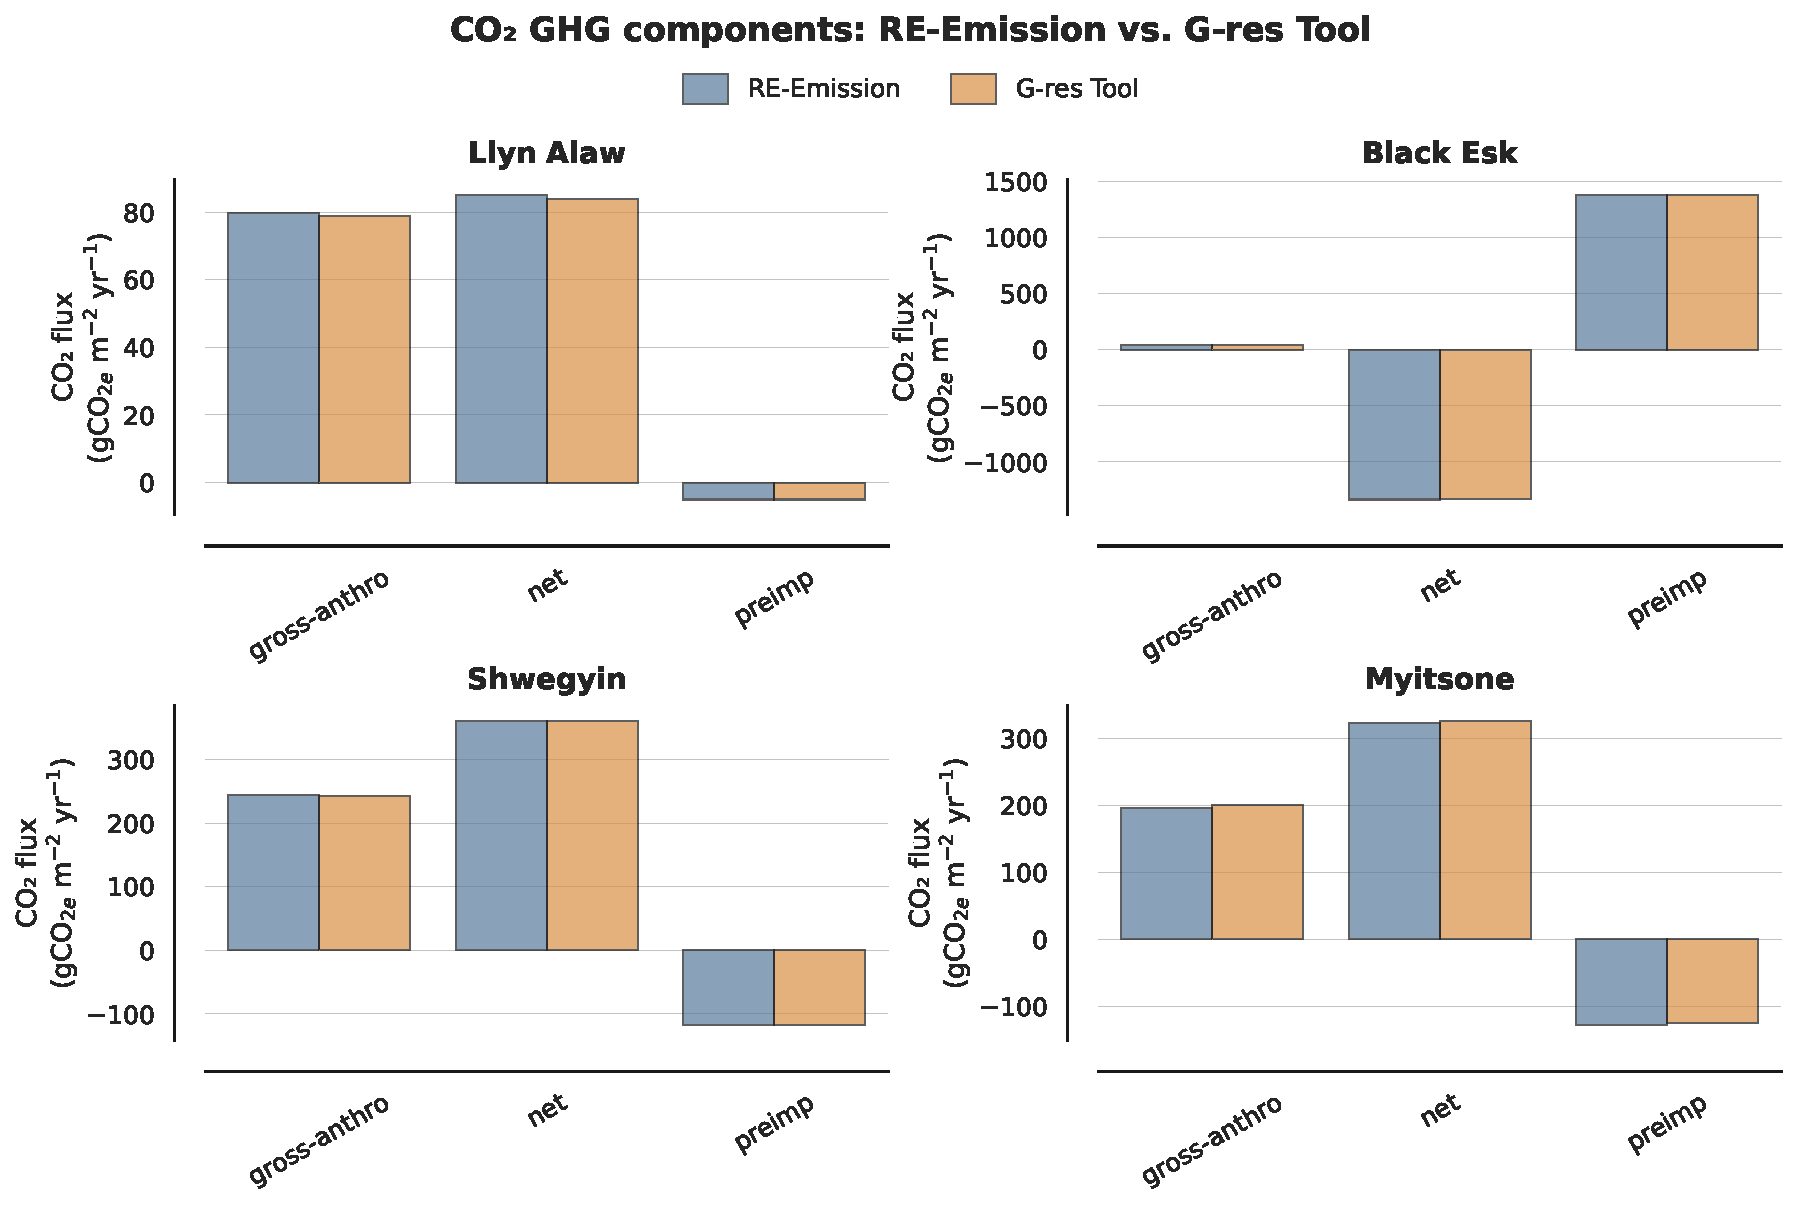
\includegraphics[width=1.0\textwidth]{figures/co2_emissions_comparison.pdf}
	\caption{Comparison of \ac{CO2} emission predictions obtained with Re-Emission and G-res Tool v3.31 for four selected reservoirs: Llyn Alaw and Black Esk (UK) and Shwegyin and Myitsone (Myanmar). Each subplot presents results for three \acs{GHG} emission components: gross anthropogenic diffusive \ac{CO2} emissions (gross-anthro), net anthropogenic \ac{CO2} emissions (net), and pre-impoundment \ac{CO2} emissions (preimp).}
    \label{supp-fig:co2_emissions_comparison}
\end{figure}


\begin{figure}[ht]
    \centering
    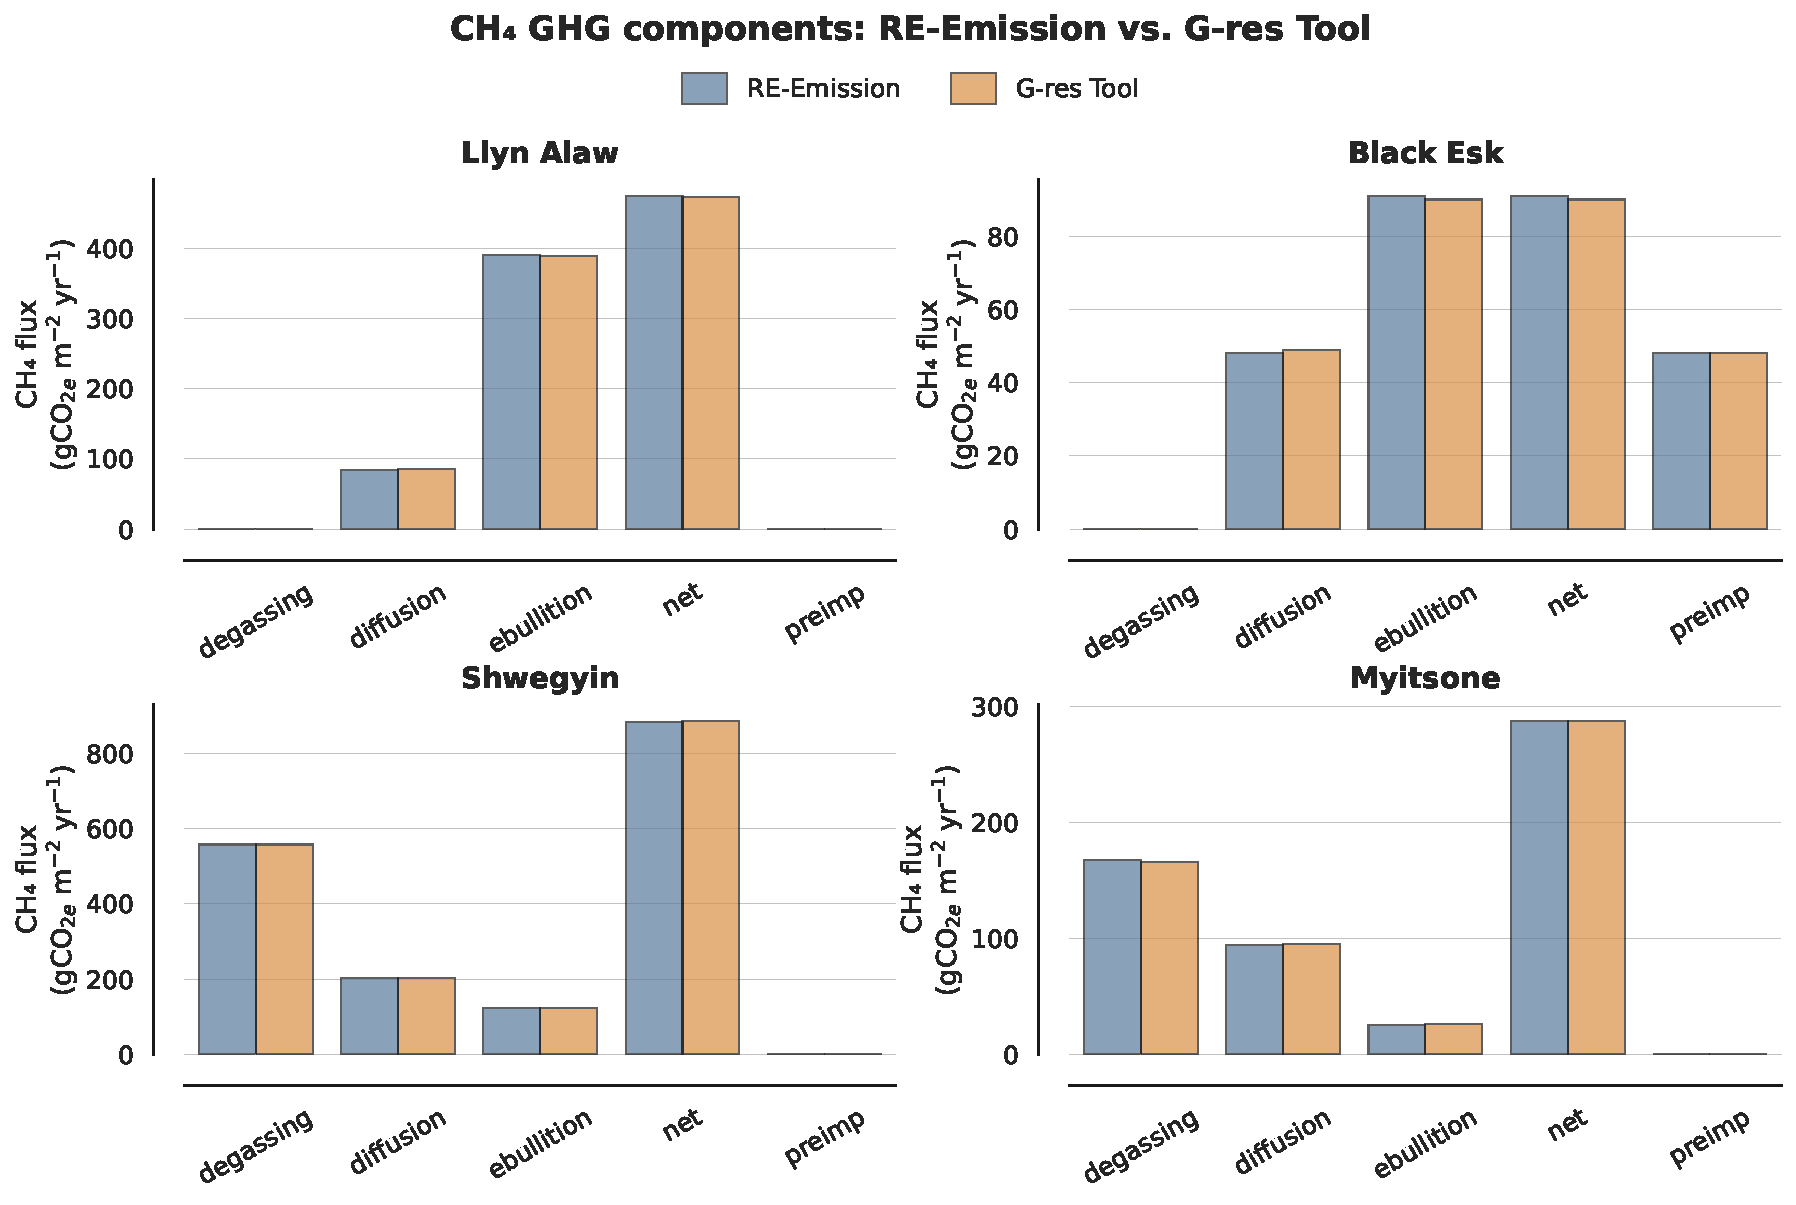
\includegraphics[width=1.0\textwidth]{figures/ch4_emissions_comparison.pdf}
	\caption{Comparison of \ac{CH4} emission predictions obtained with Re-Emissions and G-res Tool v3.31 for four selected reservoirs: Llyn Alaw and Black Esk (UK) and Shwegyin and Myitsone (Myanmar). Each subplot presents results for the following \acs{GHG} emission components: gross \ac{CH4} emissions via degassing, diffusion and ebullition respectively, net anthropogenic \ac{CH4} emissions (net), and pre-impoundment \ac{CH4} emissions (preimp).}
    \label{supp-fig:ch4_emissions_comparison}
\end{figure}

\begin{figure}[ht]
    \centering
    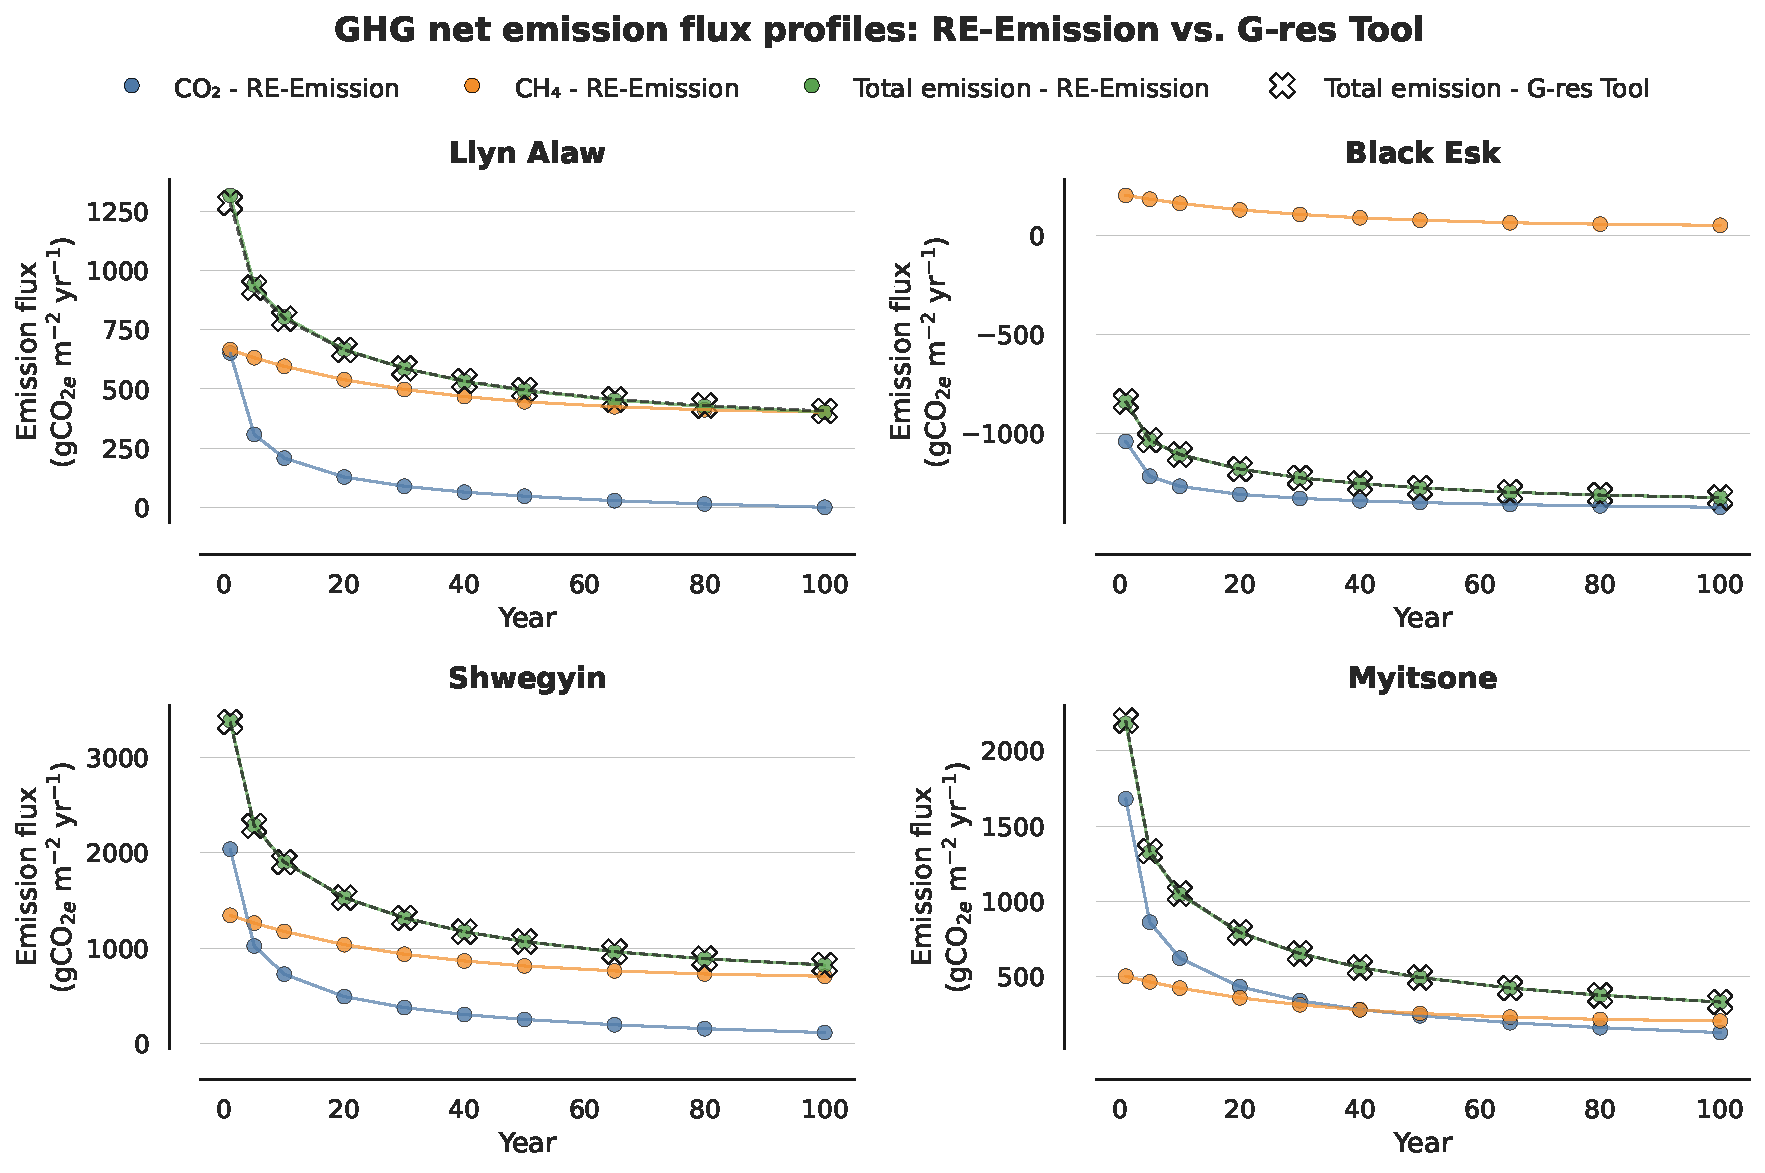
\includegraphics[width=1.0\textwidth]{figures/emissions_profile_comparison.pdf}
	\caption{Comparison of net emission flux predictions obtained with Re-Emissions and G-res Tool v3.31 for four selected reservoirs: Llyn Alaw and Black Esk (UK) and Shwegyin and Myitsone (Myanmar).}
    \label{supp-fig:emission_profile_comparison}
\end{figure}

\FloatBarrier

\begin{acronym}
	\acro{ASEAN}{Association of Southeast Asian Nations}
	\acro{BRT}{Boosted Regression Tree}
	\acro{CO2}[CO$_2$]{carbon dioxide}
	\acro{CH4}[CH$_4$]{methane}
	\acro{CI}{continuous integration}
	%\acro{CI}{carbon intensity}
	\acro{CLI}{command line interface}
	\acro{DEM}{digital elevation model}
	\acro{DOC}{dissolved organic carbon}
	\acro{DOF}{degree of fragmentation}
	\acro{DOR}{degree of regulation}
	\acro{EF}{emission factor}
	\acro{EFDC}{Environmental Fluid Dynamics Code}
	\acro{EI}{emission intensity}
	\acro{EPA}{U.S. Environmental Protection Agency}
	\acro{ET}{evapotranspiration}
	\acro{FHReD}{High-Resolution Global Database of Dams}
	\acro{FSL}{full supply level}
	\acro{GDrive}{Google Drive}
	\acro{GGRP}{Greenhouse Gas Reporting Program}
	\acro{GEE}{Google Earth Engine}
	\acro{GHCR}{GitHub Container Registry}
    \acro{GHG}{greenhouse gas}    
	\acro{GIS}{geographical information system}
	\acro{G-res}{GHG Reservoir Tool}
	\acro{GOOD2}{Global geOreferenced Database of Dams}
	\acro{GW}{gigawatts}
	\acro{HP}{hydropower}
	\acro{ICOLD}{International Commission on Large Dams}
	\acro{IHA}{International Hydropower Association}
	\acro{KDE}{kernel density estimate}
	\acro{IPCC}{Intergovernmental Panel on Climate Change}
	\acro{KNN}{K-Nearest Neighbours Regressor}
	\acro{LCA}{life-cycle assessment}
	\acro{ML}{machine-learning}
	\acro{MW}{megawatts}
	\acro{MOEA}{multiobjective evolutionary algorithm}
	\acro{MOO}{multiobjective optimization}
	\acro{N}{Nitrogen}
	\acro{N2O}[N$_2$O]{nitrous oxide}
	\acro{P}{Phosphorus}
	\acro{PD}{partial-dependence}
	\acro{PPA}{power purchase agreement}
	\acro{PV}{Photovoltaic}
	\acro{RF}{Random Forest}
	\acro{ROI}{region of interest}
	\acro{RoR}{run-of-river}
	\acro{RMSE}{root-mean-square-error}
	\acro{SA}{sensitivity analysis}
	\acro{SDG}{sustainable development goal}
	\acro{SES}{social and ecological system}
	\acro{SVR}{Support Vector Regression}
	\acro{xAI}{explainable artificial-intelligence}
	\acro{TN}{Total Nitrogen}
	\acro{TP}{Total Phosphorus}
	\acro{UAS}{Unrelated Anthropogenic Sources}
    \acro{VRE}{variable renewable energy}
	\acro{WEFE}{Water-Energy-Food-Ecosystems}
	\acro{WRT}{water residence time}
\end{acronym}

\bibliographystyle{unsrtnat}
\bibliography{reemission}

\end{document}

\endinput
%%
%% End of file `elsarticle-template-num.tex'.
